\documentclass[a4paper,11pt]{article}
\usepackage{a4wide}
\usepackage{fullpage}
\usepackage[utf8x]{inputenc}
\usepackage[slovene]{babel}
\selectlanguage{slovene}
\usepackage[toc,page]{appendix}
\usepackage[pdftex]{graphicx} % za slike
\usepackage{setspace}
\usepackage{color}
\definecolor{light-gray}{gray}{0.95}
\definecolor{green}{RGB}{0,128,0}
\usepackage{listings} % za vključevanje kode
\usepackage{hyperref}
\renewcommand{\baselinestretch}{1.2} % za boljšo berljivost večji razmak
\renewcommand{\appendixpagename}{Priloge}

\lstset{ % nastavitve za izpis kode, sem lahko tudi kaj dodaš/spremeniš
language=c++,
basicstyle=\footnotesize,
basicstyle=\ttfamily\footnotesize\setstretch{1},
backgroundcolor=\color{light-gray},
}

\title{RIS - Poročilo}
\author{Jan Gulič, Luka Podgoršek, Rok Poje, Sašo Cvitkovič}
\date{\today}

\begin{document}

\maketitle
% ----------------------------- UVOD ---------------------------------------- %
\section{Uvod}

Pri predmetu Razvoj inteligentnih sistemov (RIS) smo ekipo z imenom \textbf{team theta} sestavljali:
\begin{itemize}
	\item Cvitkovič Sašo
	\item Gulič Jan
	\item Podgoršek Luka
	\item Poje Rok
\end{itemize}

% ----------------------------- OPIS PROBLEMA ---------------------------------------- %

\section{Opis problema}

Končna naloga je bila implementacija robotskega taksija. Poligon je predstavljal mesto, v katerem se je robot vozil in izpoljeval naloge. Mesto je bilo sestavljeno iz štirih ulic, štirih hiš in prometnih znakov, katere je robot moral upoštevati med samo vožnjo. Na začetku smo robota postavili v mesto in mu sporočili njegovo lokacijo. Nato je uporabnik preko telefona (uporabljena je bila Android aplikacija) sporočil robotu svoje ime in na kateri ulici se nahaja. Robot se je odpeljal na željeno ulico in poiskal uporabnika, ki ga je poklical. Nato je s potnikom opravil kratek dialog, preko katerega je izvedel željeno destinacijo. Uporabnika je odpeljal na destinacijo, kjer je moral poiskati stavbo. Stavbe so bile predstavljene kot barvni cilindri. Po uspešni dostavi se je robot odpeljal po naslednjega uporabnika. 
Robot je nalogo opravil, ko je uspešno odpeljal tri osebe na željeno destinacijo.\\


Slike mesta, obrazev in zgradb najdete v prilogi \ref{sec:slike}{}.

% ----------------------------- REALIZACIJA ZAHTEV ---------------------------------------- %
\pagebreak
\section{Realizacija zahtev}
Zahteve, ki so obarvane z yeleno so bile realizirane.

\begin{itemize}
	\color{green}
	\item Learn the appearance of nine faces
	\item {\color{red}Learn the appearance of five traffic signs}
	\item {\color{red}Learn the appearance of four buildings}
	\item Build the map of the competition area
	\item Manually mark the streets in the map
	\item Start at any position
	\item Travel around the city
	\item {\color{red}Detect and recognize the traffic signs}
	\item {\color{red}Follow the traffic rules}
	\item Detect and recognize the faces
	\item {\color{red}Detect and recognize the buildings}
	\item Wait and understand the dispatcher's commands
	\item Ask the individuals where to take them
	\item Take the person to the correct building
	\item {\color{red}Decide whether to take two persons together}
\end{itemize}

% ----------------------------- METODOLOGIJA ---------------------------------------- %
\section{Metodologija}
\subsection{Detekcija obrazev}

Za detekcijo obrazov je uporabljen vicosov detektor.

\pagebreak
\subsection{Razpoznava obrazev}

Da je sistem lahko prepoznal obraz, smo potrebovali učne podatke. Za vsak obraz smo shranili \textbf{50 različnih slik} obraza. Te slike smo nato uporabili za izdelavo podatkovne baze z \textbf{eigenfaces}.

\begin{figure}[h]
\begin{center}
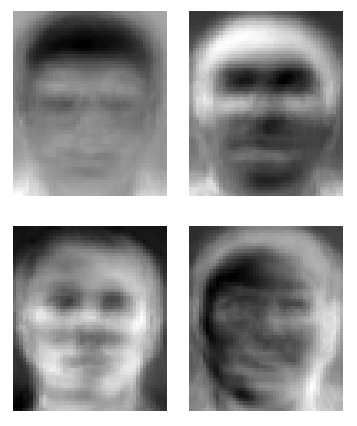
\includegraphics[scale=0.4]{Eigenfaces.png}
\caption{Primer eigenface}
\label{slika1}
\end{center}
\end{figure}

Za razpoznavo obraza je uporabljen \textbf{haarcascade} klasifikator. Ta klasifikator sta uporabila tudi Paul Viola in Michael Jones v svojem detektoju obrazev. Deluje tako, da poišče določene lastnosti na obrazu (npr. nos, oči, obrvi,...) in jih nato primerja.
//TODO Preveri

\subsection{Detekcija in razpoznava prometnih znakov}
\subsection{Detekcija in razpoznava cilindrov}
\subsection{Navigacija}

Za navigacijo robota v mapi smo uporabili podatkovno strukturo graf. Želeli smo, da robot čim hitreje pride iz točke A v točko B. Zato smo za podatkovno strukturo izbrali graf, saj poznamo algoritme za iskanje najkrajših poti v grafu.
Uporabili smo Dijkstrin algoritem za iskanje poti v grafu.

\subsubsection{Upoštevanje prometnih znakov}

Prometne znake robot upošteva s pomočjo cen povezav v grafu. Ko robot zazna prometni znak, popravi povezavo, ki vodi do tega oz. mimo tega znaka. Nrp. robot vidi znak za prepovedan promet v eno smer. Ceno povezave poveča tako, da te povezave ne bo izbral za pot, saj je ta pot neoptimalna. V primeru, da so vse ostale poti blokirane robot, ne bo upošteval prometnega znaka in prišel bo do svoje destinacije po edini možni poti.

Detekcija znaka za zvočni signal je izjema in ne popravi cene povezave. Pred tem znakom robot zatrobi.

\subsection{Dialog človek računalnik}

//TODO gulič

% ----------------------------- INTEGRACIJA ---------------------------------------- %

\section{Implementacija in integracija}

\subsection{Glavni pojmi sistema ROS}

\begin{itemize}
\item \textbf{ROS} (Robot Operation System) je odprtokodni operacijski sistem za robotiko. Vsebuje mnogo knjižnic in orodij za razvoj robotskih sistemov.
\item \textbf{Node} je samostojen proces, ki teče vzporedno z drugimi procesi.
\item \textbf{Medprocesna komunikacija} je ena izmed glavnih komponent ROS-a. Komunikacija poteka preko \textbf{tem} na katere se vežejo poslušalci in pošiljatelji. 
\item \textbf{Rviz} je orodje s katerim lahko vizualiziramo delovanje robota, mapo po kateri se premika, detektirane objekte, obraze, itd.
\end{itemize}

TODO dodaj sliko celotnega sistema

\subsection{Integracija celotnega sistema}

Naš sistem je sestavljen iz glavnega procesa in pomožnih procesov (glej sliko zgoraj). V glavnem procesu smo implementirali:
\begin{itemize}
\item Navigacijo
\item Premik do koordinat
\item Poslušalce
\item Pošiljatelje
\item Vizualizacijo delovanja
\end{itemize}

Implementacije celotnega sistema smo se lotili postopoma. Najprej smo naredili mapo celotnega mesta z uporabo Rviz-a in Kinecta ter jo shranili na disk. Sprva smo v kodo zapisali koordinate oseb, zgradb, in prometnih znakov, saj smo potrebovali testne podatke. Nato smo implementirali navigacijo in določili vozlišča grafa, ter označili posamezne ulice. Iz prejšnje naloge smo vzeli kodo za transformacijo koordinat med koordinatnimi sistemi in za premik do koordinat, ter jo dodali v nov sistem. Implementirali smo pošiljanje ti. markerjev orodju Rviz, ki je te markerje vizualiziralo. Markerji predstavljajo lokacije oseb, zgradb, prometnih znakov in vozlišč grafa. Vidna je tudi lokacija robota.

//TODO dodaj sliko RVIZA

Tako smo si pripravili osnovo samega sistema, katero je bilo možno nadgrajevati. Nato smo implementirali ostale procese, ki so skrbeli za detekcijo razpoznavo. Implementacija teh procesov je podrobno opisana v spodnjih poglavjih.

\subsection{Detekcija in razpoznava obrazev}

Za detekcijo obrazev smo uporabili \href{https://github.com/vicoslab/vicos_ros}{Vicos-ov}detektor obrazev. Detektor je uporabljen kot \textbf{ROS node}. Registriran je na temo \textbf{TODO ADD TOPIC}, kamor pošlje sporočilo v primeru detekcije obraza. Detektor vrača tudi neveljavne detekcije, zato smo v poslušalcu, ki teče v glavnem procesu implementirali filter neveljavnih detekcij.

Filter najprej omeji detekcije po višini. Imeli smo problem, saj je naš robot zaznal obraze ljudi, ki so stali ob poligonu. Ti obrazi so v danem scenariju neveljavni, povzročili pa so to, da je robot zaznal obraz na neveljavni lokaciji. V prejšnji nalogi se je robot moral zapeljati do zaznanega obraza, zato so neveljavni obrazi predstavljali problem, saj se robot ni znal zapeljati do njih in se je posledično ustavil preden je končal svojo nalogo. To smo rešili tako, da smo mu omejili vidno polje. Vse detekcije, ki so bile višje od stene poligona smo zavrgli. 

Kljub omejitvi "vidnega polja", je detektor vračal neveljavne detekcije. Npr. ročaje omare je detektor zaznal kot obraz. Zato smo v filter dodali, da more detektor zaznati obraz vsaj 5-krat v pol meterskem radiju okoli točke, kjer je bil zaznan prvi obraz. Ko detektor zazna obraz vsaj 5-krat, filter pošlje sporočilo \textbf{procesu za razpoznavo obrazev}. 

Tako kot detektor obrazev, je tudi razpoznavalec obrazev vračal napačne rešitve. To smo rešili, z dodatnim filtrom v razpoznavalcu obrazev. Razpoznavalec najprej izračuna podobnost med obrazem, ki ga vidi preko kamere in med naučenimi obrazi. V primeru, da je podobnost večja ali enaka \textbf{95\%}, poskusi razpoznati obraz. Zaradi robustnosti in izničitve napačnih razpoznav, mora razpoznavalec razpoznati obraz vsaj 10-krat. Nato pogleda kateri obraz izmed vseh obrazev je zaznal največkrat in tega označi kot veljavnega na dani lokaciji. Lokacijo veljavnega obraza pošlje orodju Rviz, ki izriše ime zaznane osebe na mapi. Lokacijo obraza prejme tudi glavni proces, ki si shrani lokacijo zaznanega obraza in jo nato uporabi pri planiranju.
 
Uporabljeni \href{http://wiki.ros.org/face_recognition}{razpoznavalec obrazev} je na voljo, kot ROS orodje. Izvorno kodo smo predelali za naše potrebe. Implementirali smo zgoraj opisani filter, popravili, da sliko prejme preko kamere in spremenili temo na kateri je poslušal. Dodali smo tudi pošiljatelja, ki je pošiljal razpoznane obraze orodju Rviz za vizualizacijo. Preden je pošiljatel poslal koordinate obraza, smo jih transformirali v koordinatni sistem mape.

\subsection{Detekcija in razpoznava prometnih znakov}

Za detekcijo objektov smo uporabili \href{https://github.com/vicoslab/vicos_ros/tree/master/detection/dlib_detector/src}{Vicos-ov} detektor. Detektor teče kot samostojen proces.

//TODO kako je uporabljen

\subsection{Detekcija in razpoznava cilindrov}

Detekcija in razpoznava cilindrov ni bila dokončno implementirana. V glavnem procesu smo ročno vnesli koordinate zgradb in jih shranili v seznam. Zaradi tega je robot lahko dostavil osebo do željene zgradbe, kljub temu, da je ni "videl". Imeli smo pripravljenega poslušalca, ki je poslušal na temi za cilindre, vendar smo to kodo zakomentirali. V primeru, da bi uspešno zaključili implementacijo detekcije cilindrov, bi poslali informacijo z koordinatami zgradbe glavnemu procesu. Glavni proces, bi nato dodal zgradbo v seznam zgradb. Seznam zgradb bi bil ob zagonu glavnega procesa prazen.

Za detekcijo cilindrov smo uporabili detektor iz knjižnice \href{http://pointclouds.org/documentation/tutorials/cylinder_segmentation.php}{PCL}. Detektor nam je vračal preveč neveljavnih detekcij, česar nismo znali odpraviti s spremembo parametrov samega orodja. V primeru, da bi detekcijo izboljšali, bi dodali še barvno preverjanje. Barvno preverjanje bi implementirali z uporabo histogramov. Sliko cilindra bi razbili na več manjših histogramov velikosti N * N in jih združili v en sam histogram. Ta histogram, bi nato uporabili za barvno primerjavo. Poleg tega bi dodali pošiljatelja, ki bi imel enako vlogo kot pošiljatel pri razpoznavi obrazev.

\subsection{\label{sec:dialog} Dialog človek robot}

//TODO gulič in šiško

\subsection{Navigacija in planiranje}

Za navigacijo v najprej znani mapi smo uporabili \textbf{graf} in algoritem \textbf{Dijkstra}. Vozlišča v grafu smo definirali v sami kodi. Vsako vozlišče vsebuje koordinate kjer se nahaja. Cene povezav med vozlišči so na začetku prazne in se posodabljajo med samim delovanjem robota. Npr. robot razpozna znak za prepovedan promet
v eno smer in popravi povezavo na kateri se nahaja znak.

Dijkstra je algoritem za iskanje najkrajših poti v grafu. Preden se robot premakne si izdela načrt, po katerih vozliščih se bo peljal. Glavni proces požene dijkstrin algoritem in izračuna najkrajšo pot do željene destinacije. Robot prejme željeno destinacijo preko glasovnih ukazov v (\ref{sec:dialog}{}) dialogu. V primeru, da robot ne ve kje se nahaja oseba ali zgradba, to osebo oz. zgradbo poišče na podani ulici. Ulice smo tako kot vozlišča v grafu, definirali v sami kodi.

\section{Delovanje celotnega sistema na tekmovanju}

//TODO dodaj po tekmovanju

% ----------------------------- PRILOGE ---------------------------------------- %
\pagebreak
\appendix
\appendixpage
\section{\label{sec:slike}Slike}
\begin{figure}[htbp]
\begin{center}

\includegraphics[width=\textwidth]{signs.png}
\caption{Veljavni prometni znaki}
\label{slika1}
\end{center}
\end{figure}

\begin{figure}[htbp]
\begin{center}
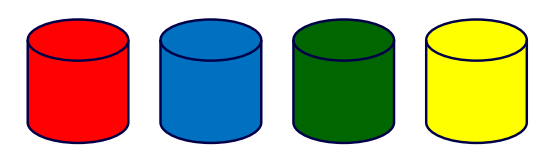
\includegraphics[width=\textwidth]{buildings.png}
\caption{Izgled zgradb}
\label{slika1}
\end{center}
\end{figure}

\begin{figure}[!tbp]
  \centering
  \begin{minipage}[b]{0.2\textwidth}
	
\includegraphics[scale=1]{city.png}
	\caption{Skica mesta}
  \end{minipage}
  \hfill
  \begin{minipage}[b]{0.2\textwidth}
	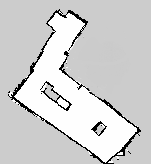
\includegraphics[scale=1]{robotMap.png}
	\caption{Mapa po kateri se je navigiral robot}
  \end{minipage}
\end{figure}


\end{document}
